%%%%%%%%%%%%%%%%%%%%%%%%%%%%%%%%%%%%%%%%%
% Journal Article
% LaTeX Template
% Version 1.3 (9/9/13)
%
% This template has been downloaded from:
% http://www.LaTeXTemplates.com
%
% Original author:
% Frits Wenneker (http://www.howtotex.com)
%
% License:
% CC BY-NC-SA 3.0 (http://creativecommons.org/licenses/by-nc-sa/3.0/)
%
%%%%%%%%%%%%%%%%%%%%%%%%%%%%%%%%%%%%%%%%%
%----------------------------------------------------------------------------------------
%       PACKAGES AND OTHER DOCUMENT CONFIGURATIONS
%----------------------------------------------------------------------------------------
\documentclass[paper=letter, fontsize=12pt]{article}
\usepackage[spanish]{babel} % Spanish language/hyphenation
\usepackage{amsmath,amsfonts,amsthm} % Math packages
\usepackage[utf8]{inputenc}
\usepackage{float}
\usepackage{lipsum} % Package to generate dummy text throughout this template
\usepackage{blindtext}
\usepackage{graphicx}
\graphicspath{{../media/}}	% Media path
\usepackage{caption}
\usepackage{subcaption}

\usepackage{tikz}
\usepackage{gantt}
\usepackage{listings}




\usepackage[sc]{mathpazo} % Use the Palatino font
\usepackage[T1]{fontenc} % Use 8-bit encoding that has 256 glyphs
\linespread{1.05} % Line spacing - Palatino needs more space between lines
\usepackage{microtype} % Slightly tweak font spacing for aesthetics
\usepackage[hmarginratio=1:1,top=32mm,columnsep=20pt]{geometry} % Document margins
\usepackage{multicol} % Used for the two-column layout of the document
%\usepackage[hang, small,labelfont=bf,up,textfont=it,up]{caption} % Custom captions under/above floats in tables or figures
\usepackage{multirow}

\usepackage{booktabs} % Horizontal rules in tables
\usepackage{float} % Required for tables and figures in the multi-column environment - they need to be placed in specific locations with the [H] (e.g. \begin{table}[H])
\usepackage{hyperref} % For hyperlinks in the PDF
\usepackage{lettrine} % The lettrine is the first enlarged letter at the beginning of the text
\usepackage{paralist} % Used for the compactitem environment which makes bullet points with less space between them
\usepackage{abstract} % Allows abstract customization
\renewcommand{\abstractnamefont}{\normalfont\bfseries} % Set the "Abstract" text to bold
\renewcommand{\abstracttextfont}{\normalfont\small\itshape} % Set the abstract itself to small italic text
\usepackage{titlesec} % Allows customization of titles

\renewcommand\thesection{\Roman{section}} % Roman numerals for the sections
\renewcommand\thesubsection{\Roman{subsection}} % Roman numerals for subsections

\titleformat{\section}[block]{\large\scshape\centering}{\thesection.}{1em}{} % Change the look of the section titles
\titleformat{\subsection}[block]{\large}{\thesubsection.}{1em}{} % Change the look of the section titles
\newcommand{\horrule}[1]{\rule{\linewidth}{#1}} % Create horizontal rule command with 1 argument of height
\usepackage{fancyhdr} % Headers and footers
\pagestyle{fancy} % All pages have headers and footers
\fancyhead{} % Blank out the default header
\fancyfoot{} % Blank out the default footer

\fancyhead[C]{Procesador con pipeline $\bullet$ Julio 2015 $\bullet$ IE521} % Custom header text

\fancyfoot[RO,LE]{\thepage} % Custom footer text
%----------------------------------------------------------------------------------------
%       TITLE SECTION
%----------------------------------------------------------------------------------------
\title{\vspace{-20mm}\hrule\vspace{5mm}\fontsize{24pt}{10pt}\selectfont\textbf{Procesador con pipeline de cinco etapas}} % Article title
\author{
\large
\href{mailto:josepabloapu@gmail.com}{\textsc{Jose Pablo Apú, B10407}}\\\href{mailto:marco.torres.810@gmail.com}{\textsc{Marco Torres, B16592}}\\\href{mailto:}{\textsc{Chuan Wu, B27371}} \\[2mm]
%\thanks{A thank you or further information}\\ % Your name
%\normalsize \href{mailto:marco.torres.810@gmail.com}{marco.torres.810@gmail.com}\\[2mm] % Your email address
\normalsize Estructuras de Computadores Digitales II \\[1mm] % Your institution
\normalsize Escuela de Ingeniería Eléctrica \\ % Your institution
\normalsize Universidad de Costa Rica \\ % Your institution
}
\date{}

%----------------------------------------------------------------------------------------
\begin{document}

\maketitle 
\hrule
%%%%%%%%%%%%%%%%%%%%%%%%%%%%%%%%%%%%%%%%%%%%%%%%%%%%%%%%%%%%% 
\begin{abstract}
En este documento se describe detalladamente el diseño, la implementación de un procesador con pipeline de cinco etapas.   
\end{abstract}

%%%%%%%%%%%%%%%%%%%%%%%%%%%%%%%%%%%%%%%%%%%%%%%%%%%%%%%%%%%%%
\section{Introducción}

\subsection{Desarrollo del proyecto}

Se pretende describir un microprocesador con pipeline de cinco etapas. Las características principales son:

\begin{enumerate}
\item No tendrá direccionamiento indirecto.
\item Tendrá dos registros de uso general, llamados A y B.
\item No se harán operaciones de A con Memoria, ni de B con Memoria, únicamente entre A, B y constantes.
\item La memoria de datos estará separada de la de instrucciones.
\item Cada posición de la memoria de datos guardará un byte.
\item Cada posición de la memoria de instrucciones guardará dos bytes.
\item La memoria de datos tendrá 1024 posiciones (10 bits para indexarla).
\item La memoria de instrucciones tendrá 1024 posiciones (10 bits para indexarla).
\item No habrá subrutinas.
\item No se implementará atención a interrupciones.
\item No se implementará una pila.
\item Se supondrán únicamente números sin signo, por lo que no habrá bandera de rebase.
\end{enumerate}

\subsection{Plan de pruebas}

Con la tabla de instrucciones, que se pueden observar en el cuadro \ref{tablaDecodificacion}, se piensa contruir pogramas pequeños, pero característicos, esto para observar el comportamiento del microprocesador.

\section{Diseño}

El que tenga un pipeline, permite estar ejecutando una intrucción, y que en ese momento pueda recibir otra intrucción. Sabemos que las intrucciones por lo general, necesitan de 2 a 3 ciclos de reloj. La idea es que al ejecutarse el segundo ciclo de reloj, el procesador pueda recibir la siguiente instrucción, sin que la primera instrucción finalice. Para lograr esto hay que definir muy bien cada bloque, así como tener mucho cuidado con las propagación de las señales.

\subsection{Decodificador}
El microprocesador tiene una unidad de control, que es este caso se llama decodificador. Este permite administrar las entradas que recibe la alu, los regirstros y además maneja los saltos del microprocesador.

Los principales componentes son:

\subsection{ALU}
Es el encargado se hacer operacioneces aritméticas y lógicas, además nos ayuda a pasar datos a la RAM. Es un circuito combinacional por lo que no ocupa de reloj.

\subsection{Registros}
Además de funcionar como un flip-flop. Este tiene como comportamiento predeterminado mantener su salida anterior. Pero esta puede ser cambiada por el decodificador.

\subsection{RAM y ROM}
Ambas son memorias, nada más que la primera es solo lectura y la segundo si se puede escribir. Estan separadas, y la ROM es la que tiene el pograma ensamblado y la RAM es con el cual el microprocesador guarda y lee datos para hacer sus distintas operaciones.

\section{Definición de la máquina}

\subsection{Multiplexores}

\begin{table}[h]
\centering
\begin{tabular}{cc|cc}
\multicolumn{4}{c}{Sistema de control} \\ \hline
selM1 & selM2 & ln1 	& ln2  \\ \hline
0     & 0     & wA 	& imdt \\
0     & 1     & wA	& wB   \\
1     & 0     & imdt	& imdt \\
1     & 1     & imdt	& wB   \\
\end{tabular}
\end{table}

\subsection{Acumulador}

\begin{table}[h]
\centering
\begin{tabular}{c|c}
\multicolumn{2}{c}{Sistema de control} \\ \hline
selX   & wX    \\ \hline
00     & wX    \\
01     & inmdt \\
10     & alu   \\
11     & mem   \\
\end{tabular}
\end{table}

\subsection{Decodificador}

\begin{itemize}
\item \textbf{Entradas:}\\
instr
\item \textbf{Salidas:}\\
selA, selB, selM1, selM2, inm, memDir, branchDir, jmpDir, jmpTaken, wrEnable, opCode
\item \textbf{Asignaciónes:} \\
inm = instr[0:7] \\
memDir = jmpDir = instr[0:9] \\
branchDir = instr[0:5] \\
opCode = instr[10:15]
\end{itemize}

En la tabla \ref{tablaDecodificacion} se observa las salidad de control, que hace el decodificador para manejar los registros y los muxes que van hacia la alu.

\begin{table}
\centering
\begin{tabular}{cc|ccccc}
\multicolumn{7}{c}{Salida según la intrucción} \\ \hline
Codificación& Mnemónico	  	& selA & selB & selM1 & selM2 & wrEnable \\ \hline
000 000 	& LDA 		  	& 11 	& 00    & X     & X     & 0 \\
000 001		& LDB  			& 00 	& 11    & X     & X     & 0 \\           
000 010 	& LDCA 			& 01 	& 00    & X     & X     & 0 \\            
000 011 	& LDCB 			& 00 	& 01    & X     & X     & 0 \\           
000 100 	& STA  	 		& 00 	& 00    & 0     & X     & 1 \\            
000 101 	& STB  			& 00 	& 00    & X     & 0     & 1 \\            
000 110 	& ADDA			& 10 	& 00    & 0     & 1     & 0 \\
000 111 	& ADDB			& 00 	& 10    & 0     & 1     & 0 \\
001 000 	& ADDCA			& 10 	& 00    & 0     & 0     & 0 \\
001 001 	& ADDCB			& 00 	& 10    & 1     & 1     & 0 \\
001 010 	& SUBA			& 10 	& 00    & 0     & 1     & 0 \\
001 011 	& SUBB			& 00 	& 10    & 0     & 1     & 0 \\
001 100 	& SUBCA			& 10 	& 00    & 0     & 0     & 0 \\
001 101 	& SUBCB			& 00 	& 10    & 1     & 1     & 0 \\
001 110 	& ANDA			& 10 	& 00    & 0     & 1     & 0 \\
001 111 	& ANDB			& 00 	& 10    & 0    	& 1     & 0 \\
010 000 	& ANDCA			& 10 	& 00    & 0     & 0     & 0 \\
010 001 	& ANDCB			& 00 	& 10    & 1     & 1     & 0 \\
010 010 	& ORA			& 10 	& 00    & 0     & 1     & 0 \\
010 011 	& ORB			& 00 	& 10    & 0     & 1     & 0 \\
010 100 	& ORCA			& 10 	& 00    & 0     & 0     & 0 \\
010 101 	& ORCB			& 00 	& 10    & 1     & 1     & 0 \\
010 110 	& ASLA			& 10 	& 00    & X     & X     & 0 \\
010 111 	& ASRA			& 10 	& 00    & X     & X     & 0 \\
	
011 000 	& JMP			& 00 	& 00    & X     & X     & 0 \\
011 001 	& BAEQ			& 00 	& 00    & X     & X     & 0 \\
011 010 	& BANE			& 00 	& 00    & X     & X     & 0 \\
011 011 	& BACS			& 00 	& 00    & X     & X     & 0 \\
011 100 	& BACC			& 00 	& 00    & X     & X     & 0 \\
011 101 	& BAMI			& 00 	& 00    & X     & X     & 0 \\
011 110 	& BAPL			& 00 	& 00    & X     & X     & 0 \\
011 111 	& BBEQ			& 00 	& 00    & X     & X     & 0 \\
100 000 	& BBNE			& 00 	& 00    & X     & X     & 0 \\
100 001 	& BBCS			& 00 	& 00    & X     & X     & 0 \\
100 010 	& BBCC			& 00 	& 00    & X     & X     & 0 \\
100 011 	& BBMI			& 00 	& 00    & X     & X     & 0 \\
100 100 	& BBPL			& 00 	& 00    & X     & X     & 0 \\

100 101 	& NOP			& 00 	& 00    & X     & X     & 0 \\

\end{tabular}
\caption{Salidas de control, del decodificador}
\label{tablaDecodificacion}
\end{table}


\subsection{Memoria de datos}

\subsection{Memoria de instrucciones}

\pagebreak
%%%%%%%%%%%%%%%%%%%%%%%%%%%%%%%%%%%%%%%%%%%%%%%%%%%%%%%%%%%%%
\section{Implementación}

\begin{figure}[hbtp]
\centering
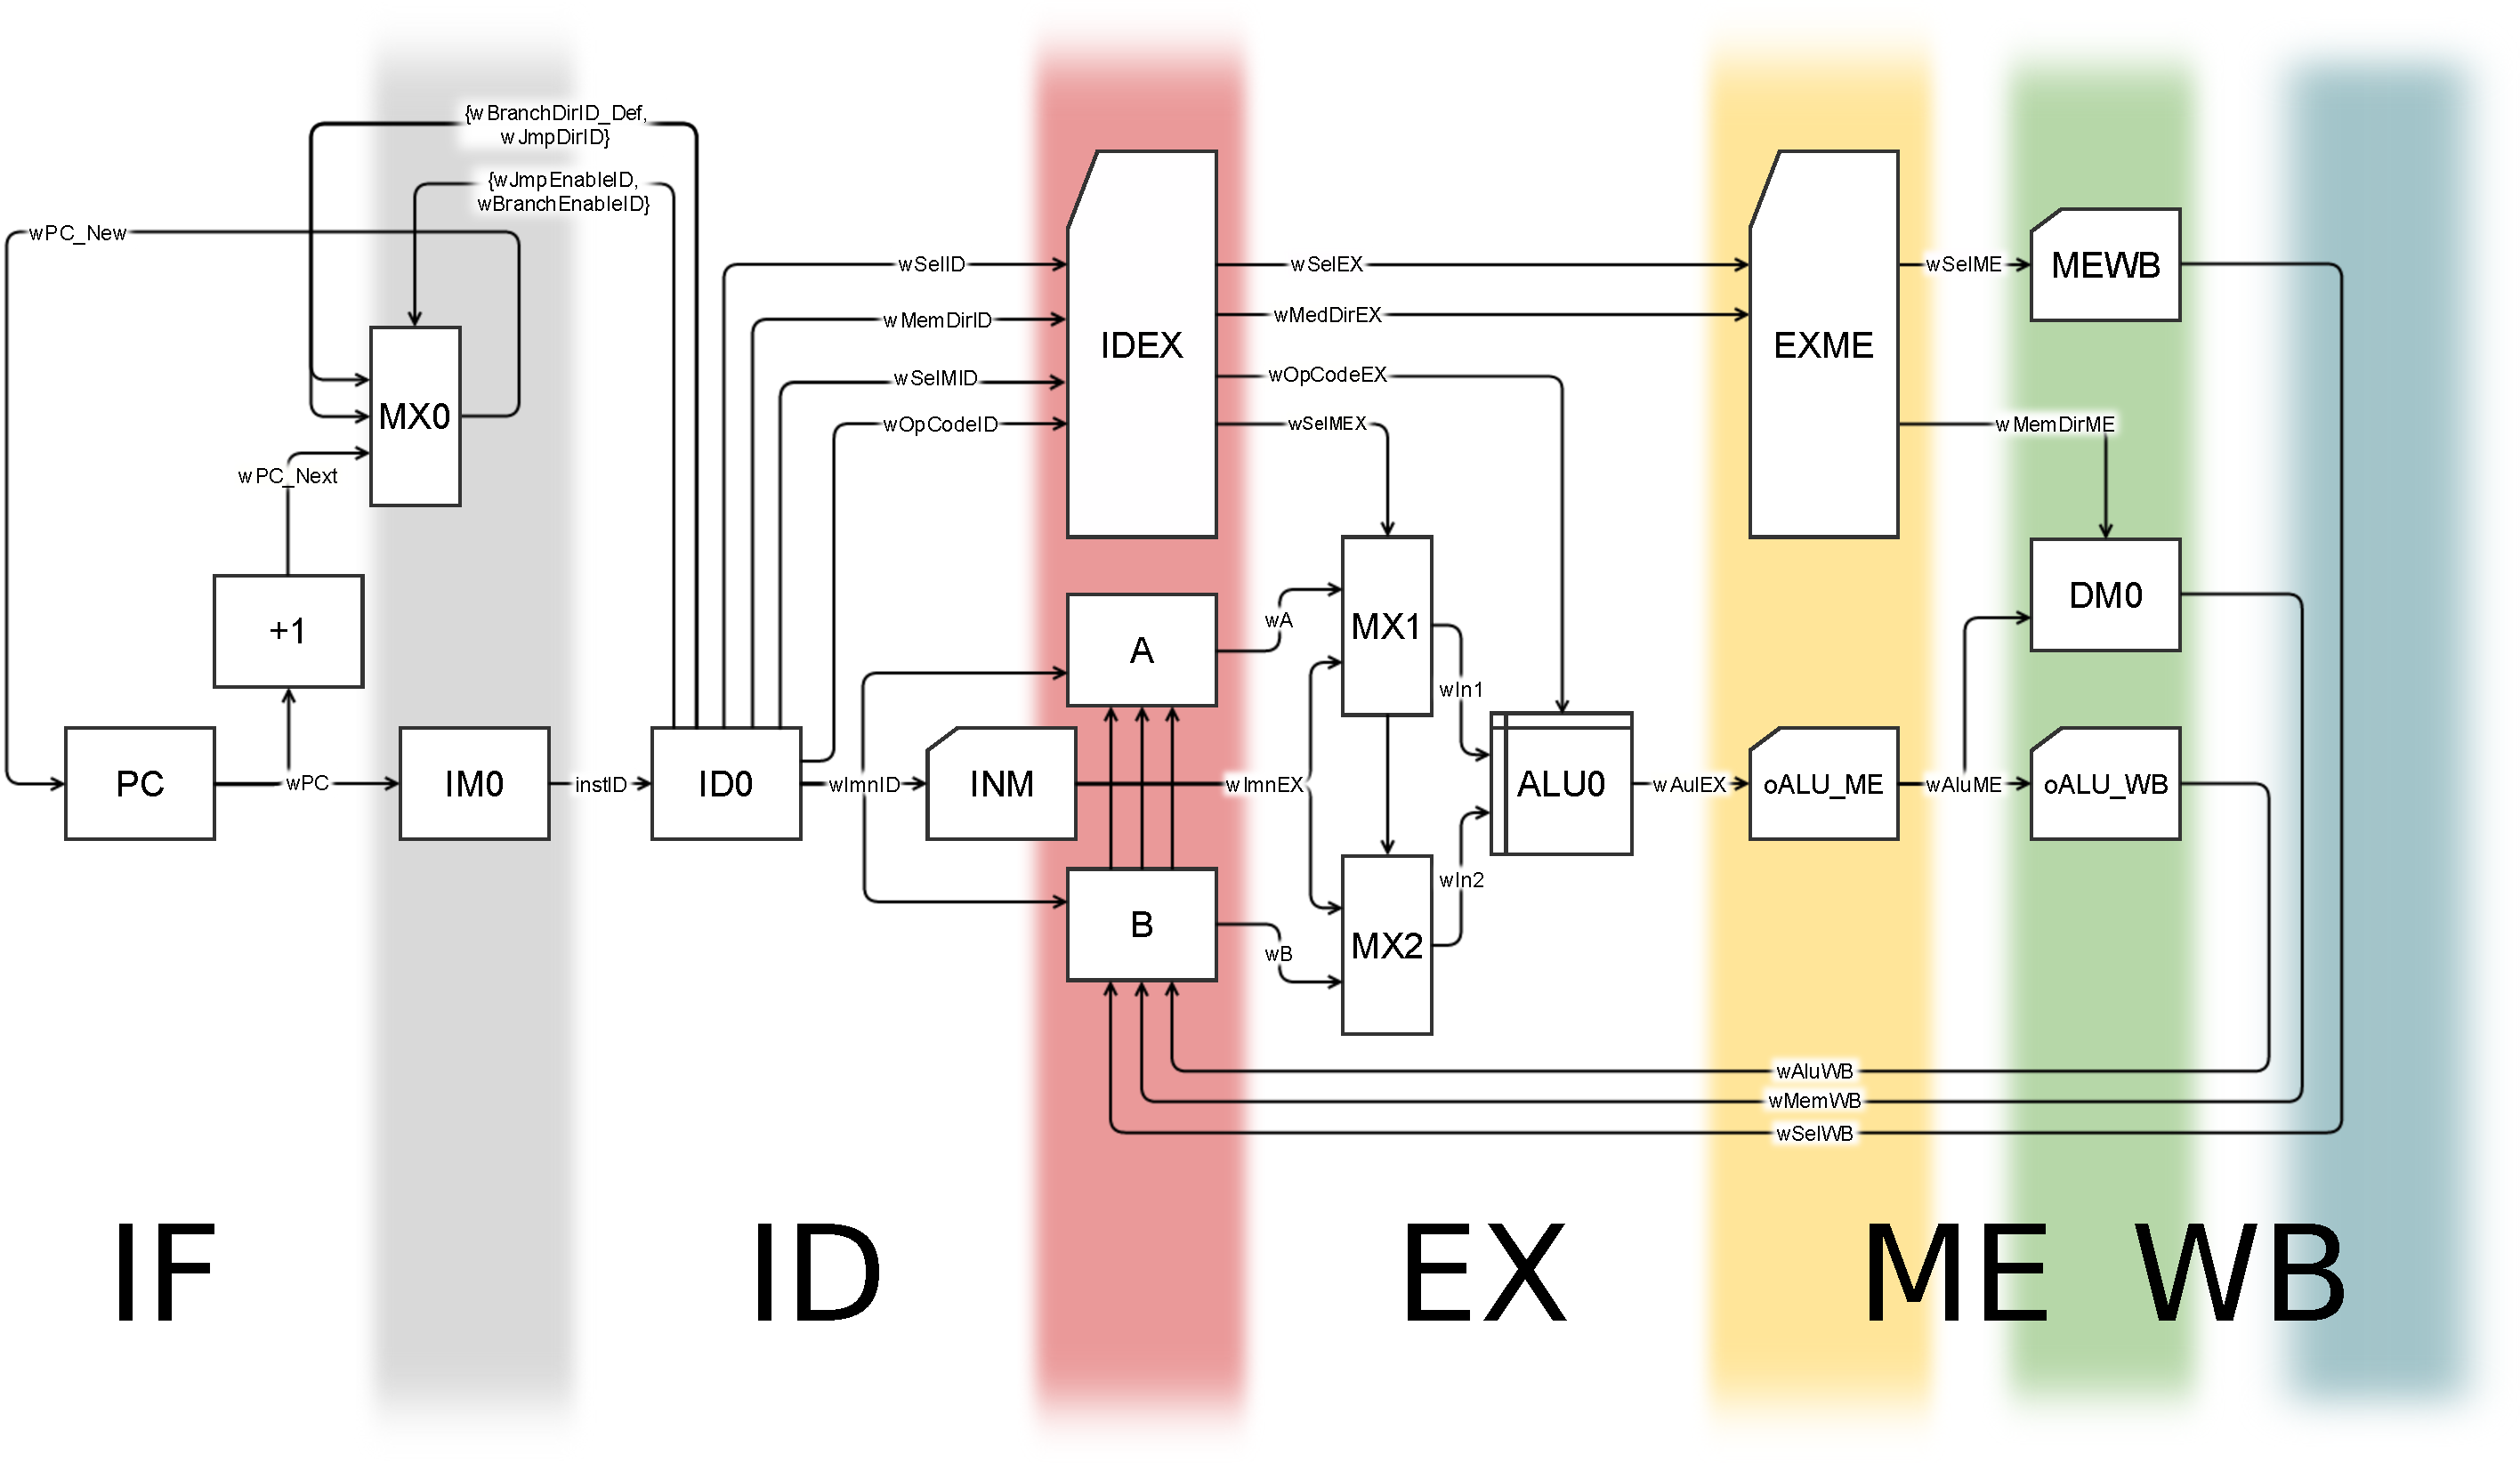
\includegraphics[width=1\linewidth]{araucaria_pipeline}
\caption{Plan de pruebas}
\end{figure}

%%%%%%%%%%%%%%%%%%%%%%%%%%%%%%%%%%%%%%%%%%%%%%%%%%%%%%%%%%%%%
\section{Verificación y plan de pruebas}

Asi como se menciona en la introducción para validar el diseño se ejecuto el plan de pruebas. Acontinuacion se listan cada una de las prubas que se realizaron una vez que se comprobó que cada elemento fuincionaba individualmente.

\subsection{Operaciones aritméticas y de carga de constantes}
Para esta prueba se propuso la creacion de un programa que tomara dos numeros constante, los restara y luego sumara otro. Acontinuacion se muestra el código en lenguaje ensamblador.

\begin{lstlisting}
		#Programa 1:
NOP
LDCA 9A			#Se carga un $9A al acomulador A
NOP
NOP
LDCB 2C			#Se carga un $2C al acomulador B
NOP
NOP
SUBA			#(A) <- (A)-(B)
NOP
NOP
ADDCA 14		#(A) <- (A) + ($14)
NOP
NOP
		###
\end{lstlisting}

En la figura \ref{i:p1} se muestra el resultado de correr este programa el tiempo suficiente para que todas las instrucciones pasen por las etapas.\\

\begin{figure}[hbtp]
\centering
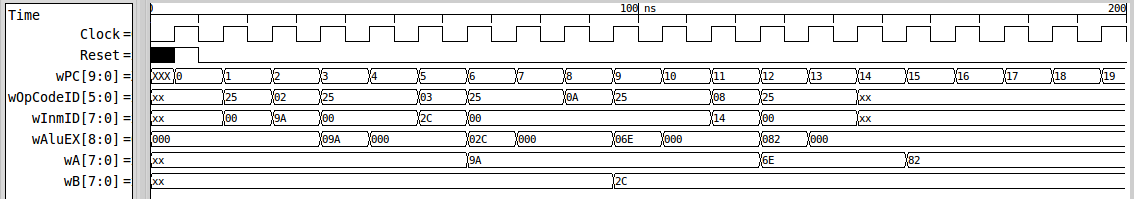
\includegraphics[width=1\linewidth]{../test/Prog1.png}
\caption{Señales de control y datos durante la ejecucion de programa 1.}
\label{i:p1}
\end{figure}

Vale la pena prestar atencion a la linea \textbf{wOpCodeID} pues esta dice cual instrucccion se acaba de decodificar, tambien es importante ver a linea \textbf{wAluEX} pues esta muestra la salida de la \textit{ALU}, en este caso los valores inmediatos que se van almacenar, finalmente al detallar las lineas \textbf{wA} y \textbf{wB} se puede ver el resultado de las instrucciones que se estan ejecutando. Adicionalmente aunque no se muestren las demas señales de control se verifico que fueran las correctas, por lo cual podemos comprobar el resultado de la operacion \ref{e:p1}.\\

\begin{align} 
\label{e:p1}
(\$9A - \$2C) + \$12 = \$14
\end{align}

\subsection{Acceso a memoria (lectura y escritura)}

Para probar el funcionamiento de las instrucciones de acceso a memoria basto con guardar el contenido del acomulador en una posicion de memoria y luego cargarlo desde la memoria a otro acomulador. Acontinuacion se muestra el código en lenguaje ensamblador.

\begin{lstlisting}
		#Programa 2:
NOP
LDCA 9A			#Se carga un $9A al acomulador A
NOP
NOP
STA 100			#Se guarda el contenido de A 
NOP			#en la posicion $100 de la memoria
NOP
LDB 100			#Se carga al acomulador B el 
NOP			#contenido de la posicion $100
NOP
		###
\end{lstlisting}

En la figura \ref{i:p2} se muestran las señales al ejecutar este programa.\\

\begin{figure}[hbtp]
\centering
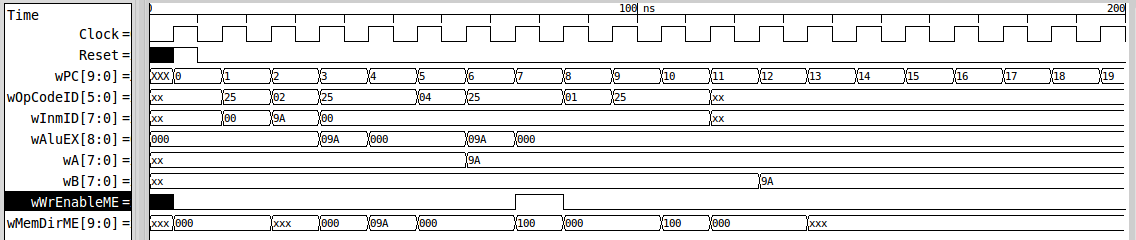
\includegraphics[width=1\linewidth]{../test/Prog2.png}
\caption{Señales de control y datos durante la ejecucion de programa 2.}
\label{i:p2}
\end{figure}

En este caso tambien es importante detallar las lineas \textbf{wA}, \textbf{wB} \textbf{wAluEX} y \textbf{wOpCode}, pero por el objetivo de la prueba se centro el analisis en las lineas \textbf{wWrEnableME} y \textbf{wMemDirME}. Para todos los casos la memoria siempre esta cargando en la salida el contenido de la posicion de memoria que indica wMemDirME pero solo escribe lo que esta su entrada cuando la linea wWrEnable esta en alto. Finalmente se puede comprobar que las instrucciones se ejecutaron bien observando la lina \textbf{wB} al final de la ejecucion.

\clearpage
\subsection{Operaciones lógicas}

En el caso de las operaciones lógicas se hizo un programa que tomara un numero y le quitara los cuatro bits menos significativos y luego desplazara los cuatro bits mas significativos cuatro veces a la derecha.Acontinuacion se muestra el código en lenguaje ensamblador.

\begin{lstlisting}
			#Programa 3:
NOP
LDCA 9A		#Se carga un $9A al acomulador A
NOP
NOP
LDCB F0		#Se carga un $F0 al acomulador B
NOP
NOP
ANDA		#Se hace un AND bit por bit entre los acomuladores
NOP
NOP
ASRA		#Se rota una vez a la derecha el acomulador A
NOP
NOP
ASRA
NOP
NOP
ASRA		#Se rota una vez a la derecha el acomulador A
NOP
NOP
ASRA		#Se rota una vez a la derecha el acomulador A
NOP
NOP
			###
\end{lstlisting}

En la figura \ref{i:p3} se muestran las señales al ejecutar este programa.\\

\begin{figure}[hbtp]
\centering
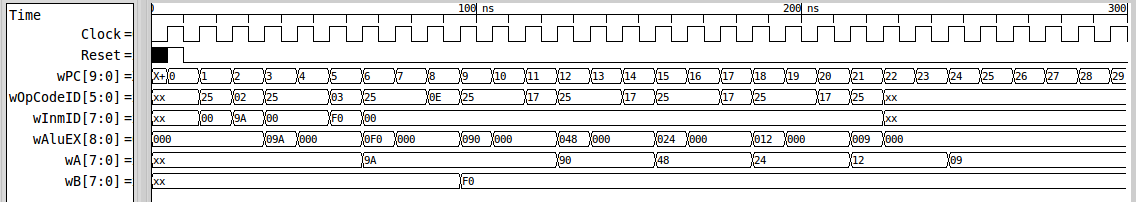
\includegraphics[width=1\linewidth]{../test/Prog3.png}
\caption{Señales de control y datos durante la ejecucion de programa 3.}
\label{i:p3}
\end{figure}

Aqui solamente vale la pena resaltar el contenido en las lineas \textbf{wOpCodeID} que muestra la instruccion a ejecutar y la linea \textbf{wA} que muestra el resultado del contenido del acomulador despues de ejecutar las intrucciones lógicas. Ademas es posible confirmar el resultado haciendo los calculos a mano \ref{e:p3}.

\begin{align} 
\label{e:p3}
\$9A  (AND) \$F0 = \$90 \\
(\$90) >> 4 = \$09
\end{align}


\subsection{Control de flujo | Saltos incondicionales}

Para los saltos incondicionales solo se tuvo que interrumpir la linea del contador de programa y que siguiera en otro lado, por eso se hizo un programa que cargara un numero al acomulador A y mas adelante lo alterara pero antes de eso se coloco un salto incondicional de modo que si el salto funcionaba el dato no seria alterado. Acontinuacion se muestra el código en lenguaje ensamblador.

\begin{lstlisting}
		#Programa 4:
NOP
LDCA 05			#Se carga al acomulador A un $05
NOP
NOP
JMP J1 :		#Se salta a la posicion indicada por J1
NOP
NOP
LDCA FF			#Se carga al acomulador A un $FF
NOP			#(este codigo no se ejecuta)
NOP
: J1 :			#Etiqueta de Salto 1
NOP
NOP
NOP
NOP
NOP
NOP
		###
\end{lstlisting}

En la figura \ref{i:p4} se muestran las señales al ejecutar este programa.\\

\begin{figure}[hbtp]
\centering
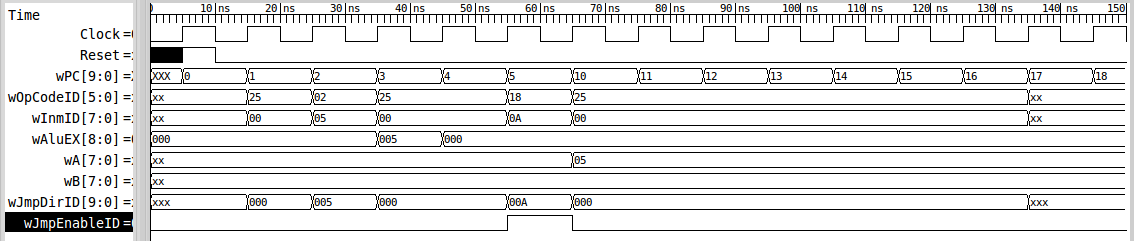
\includegraphics[width=1\linewidth]{../test/Prog4.png}
\caption{Señales de control y datos durante la ejecucion de programa 4.}
\label{i:p4}
\end{figure}

Para esta prueba es de mucha importancia observar las lineas \textbf{wPC}, \textbf{wJmpEnableID} y \textbf{wJmpDirID} porque si bien la linea de direccion de salto siempr mustra algun valo solo se salta a este cuando el habilitador esta arriba. Se puede ver facilmente que la instruccion funciona bien al observar el contador de programa en \textbf{wPC}.

\subsection{Control de flujo | Saltos condicionales}

Para los saltos condicionales se hizo un programa que cargara un numero en el acomulador A y otro en el acomulador B. Luego desplazaria hacia la izquierda el numero en A tantas veces como induque el numero en B. Acontinuacion se muestra el código en lenguaje ensamblador.

\begin{lstlisting}
		#Programa 5:
NOP
LDCA 01			#Se carga un 1 en el acomulador A
NOP
NOP
LDCB 3			#Se carga un 3 en el acomulador B
: J2 :			#Etiquita de Salto 2
NOP
NOP
ASLA			#Se desplaza hacia la izquierda el numero en A
NOP
NOP
SUBCB 1			#Se decrementa el numero en B
NOP
NOP
NOP
BBNE J2 :		#Si el numero en B no es cero se 
NOP			#salta a la etiqueta
NO
		###
\end{lstlisting}

Para verificar el funcionamiento de este programa se deben observar las lineas \textbf{wPC}, \textbf{wA}, \textbf{wB} y \textbf{wBranchEnableID} y facilmente se puede observar el resultado que se muestra en la linea wA para verificar el resultado \ref{e:p5}.

\begin{align} 
\label{e:p5}
(\$01) >> 3 = \$08
\end{align}

EN otra prueba.. CHUAN AQUÍ VA UNA SUYA

\clearpage
\section{Conclusiones y recomendaciones}

\begin{itemize}
\item Apezar de que no se exploto al máximo el "pipeline" se logro diseñar e implementar un procesador completamente funcional que ejecutara programas y almacenara los resultados.\\


\item Como en el diseño solo se implemento con las señales de control y datos basicas el procesador no puede evitar o reducir "hazards" de ningun tipo, esto por falta de tiempo para implementar esta funcionalidad. A pesar de esto aqui se comenta como se planeo ampliar el diseo para soportar esta funcionalidad.\\

\item Al ejecutar una instrucccion de salto, ya sea condicional o incondicional el contador de programa se incrementa pues aun no se ha decodificado la instruccion, esto causa que se lea la siguiente instruccion despues de la de salto. Para solucionar esto se planeo implementar un modulo que controlara el contenido de los registros de "pipe", de este modo cuando se leyera la siguiente instruccion el modulo reiniciaria el registro de "pipe" IF/ID para convertir la instrucccion leida en un NOP.\\

\item Tambien por la forma en la que se diseño la etapa WB, si se ejecuta una instruccion que lea el acomulador A luego de una que lo escriba el valor leido sera un valor viejo. Para preveer este problema se debe crear un modulo que controle los registros de "pipe" de modo que pueda detener algunas etapas para empezar a introducir burbujas en las etapas que tienen el problema.\\

\item Finalmente vale la pena agregar que aunque puede llegar a ser muy complejo diseñar un procesador, en general si se modulariza de la forma correcta y se verifica cada parte por separado la mayor parte del diseño se vuelve facil de diseñar.
\end{itemize}

\end{document}